\documentclass[12pt, a4paper]{article}

\usepackage{fancyhdr}
\usepackage[left=4cm, right=4cm, top=4cm, bottom=4cm]{geometry}
\usepackage[utf8]{inputenc}
\usepackage[table]{xcolor}
\usepackage{hyperref}
\usepackage{amsmath}
\usepackage{enumitem}
\usepackage{graphicx}
\usepackage{booktabs}
\usepackage{subcaption}
\usepackage[justification=centering]{caption}
\usepackage[most]{tcolorbox}
\usepackage{xepersian}

\DeclareMathOperator*{\argmax}{argmax}
\DeclareMathOperator*{\argmin}{argmin}
\newcolumntype{L}{>{$}l<{$}} % math-mode version of "l" column type

\newcommand{\coursetitle}{پردازش زبان طبیعی}
\newcommand{\doctitle}{تمرین دوم}
\newcommand{\name}{محمدرضا غفرانی}
\newcommand{\studentno}{400131076}
\newcommand{\todaydate}{\today}

\settextfont{XB Kayhan}
\setlatintextfont{Times Newer Roman}

\pagestyle{fancy}
\lhead{\textbf{\doctitle}}
\chead{\name}
\rhead{\todaydate}

\begin{document}

\begin{flushleft}
    \name \\
    \studentno \\
    \todaydate
\end{flushleft}

\begin{center}
    \huge
    \textbf{\coursetitle}
    \break
    \large
    \doctitle
\end{center}

% suppress the fancy header on the first page only
\thispagestyle{plain}

\section*{بخش اول}

\subsection*{گام سوم}

در جدول \ref{similar_documents} شبیه‌ترین مستند به اسناد گفته شده مشاهده می‌شود.
به طور کلی درصد شباهت نسبت داده شده توسط ترکیب دو روش \lr{TF-IDF} و \lr{Word2vec}
بیشتر از مدل \lr{Doc2vec} است.

\begin{latin}
    \begin{table}[h]
        \caption{\rl{شناسه‌های شبیه‌ترین مستندات به اسناد گفته شده}}
        \label{similar_documents}
        \begin{tabular}[]{l|l|l||l|l}
            & \multicolumn{2}{c||}{TF-IDF \& Word2vec} & \multicolumn{2}{c}{Doc2Vec} \\ \hline
             & Similar Doc & Similarity & Similar Doc & Similarity \\ \hline
            Doc1  & Doc165 & 0.98 & Doc33  & 0.69 \\
            Doc3  & Doc19  & 0.99 & Doc19  & 0.85 \\
            Doc5  & Doc26  & 0.98 & Doc0   & 0.62 \\
            Doc25 & Doc679 & 1    & Doc679 & 0.99 \\
            Doc36 & Doc7   & 0.98 & Doc0   & 0.61
        \end{tabular}
    \end{table}
\end{latin}

همچنین روش \lr{TF-IDF\&Word2vec} مستندات شبیه‌تری را
خروجی برمی‌گرداند. برای مثال برای مستند \lr{Doc5} روش \lr{TF-IDF\&Word2evc} مستند با شناسه
\lr{Doc26} را بازگردانده است در حالی که روش \lr{Doc2vec} مستند \lr{Doc0} را بازگردانده است.
با بررسی این مستندات مشخص است که مستند \lr{Doc26} از نظر محتوایی نسبت به
سند \lr{Doc0} به مستند \lr{Doc5} بسیار شبیه‌تر است.

\pagebreak

\subsection*{گام چهارم}

در جدول \ref{similar_words} شبیه‌ترین کلمه به هر یک از کلمات داده شده مشاهده می‌شود.
کلمه‌های مشابه و درصد شباهت هر کلمه به نظر معقول می‌رسد. در کلماتی نظیر «استقلال» که
کلمه چندین معنا دارد، کلمات از حوزه‌های مختلف آورده شده است.

\begin{table}[h]
    \caption{شبیه‌ترین واژگان به کلمات داده شده}
    \label{similar_words}
    \hfil
    \begin{tabular}{c|c}
        \multicolumn{2}{c}{\cellcolor{blue!25}تهران} \\[5pt]
        کلمه & درصد شباهت \\  \hline
        کرج & 0.60 \\
        اصفهان & 0.60 \\
        تبریز & 0.59
    \end{tabular}
    \hfil
    \begin{tabular}{c|c}
        \multicolumn{2}{c}{\cellcolor{blue!25}بهداشت} \\[5pt]
        کلمه & درصد شباهت \\ \hline
        باروری & 0.79 \\
        مراقبت‌های & 0.75 \\
        بهداشتی & 0.73
    \end{tabular}
    \\[10   pt]
    \smallskip
    \hfil
    \begin{tabular}{c|c}
        \multicolumn{2}{c}{\cellcolor{blue!25}دفاع} \\[5pt]
        کلمه & درصد شباهت \\ \hline
        مقدس & 0.68 \\
        پشتیبانی & 0.66 \\
        ضدموشکی & 0.64
    \end{tabular}
    \hfil
    \begin{tabular}{c|c}
        \multicolumn{2}{c}{\cellcolor{blue!25}رودخانه} \\[5pt]
        کلمه & درصد شباهت \\ \hline
        دریاچه & 0.86 \\
        کارون & 0.85 \\
        ارتفاعات & 0.84
    \end{tabular}
    \\[10   pt]
    \smallskip
    \hfil
    \begin{tabular}{c|c}
        \multicolumn{2}{c}{\cellcolor{blue!25}سرد} \\[5pt]
        کلمه & درصد شباهت \\ \hline
        زمستان‌های & 0.78 \\
        زمستان & 0.78 \\
        مرطوب & 0.77
    \end{tabular}
    \hfil
    \begin{tabular}{c|c}
        \multicolumn{2}{c}{\cellcolor{blue!25}فرهنگ} \\[5pt]
        کلمه & درصد شباهت \\ \hline
        ارشاد & 0.79 \\
        سمعی & 0.71 \\
        تجسمی & 0.68
    \end{tabular}
    \\[10   pt]
    \smallskip
    \hfil
    \begin{tabular}{c|c}
        \multicolumn{2}{c}{\cellcolor{blue!25}استقلال} \\[5pt]
        کلمه & درصد شباهت \\ \hline
        پاس & 0.68 \\
        ارضی & 0.68 \\
        پیکان & 0.67
    \end{tabular}
    \hfil
\end{table}

در شکل‌های \ref{embedding_diagram} نمودار بردار تعبیه کلمات با کاهش ابعاد بردار به ۲ و ۳ بعد رسم شده است.
همان‌طور که انتظار داشتیم کلمات مشابه به یکدیگر در کنار یکدیگر قرار دارند. همچنین کلماتی از دسته‌های مختلف
که به هم نزدیک هستند نیز در نزدیکی یکدیگرند قرار گرفته‌اند. با افزایش بعد داده‌ها می‌توان با دقت
بیشتر شهود بهتری را می‌توان از کلمات به دست آورد.

\begin{figure}
    \begin{subfigure}{0.45\linewidth}
        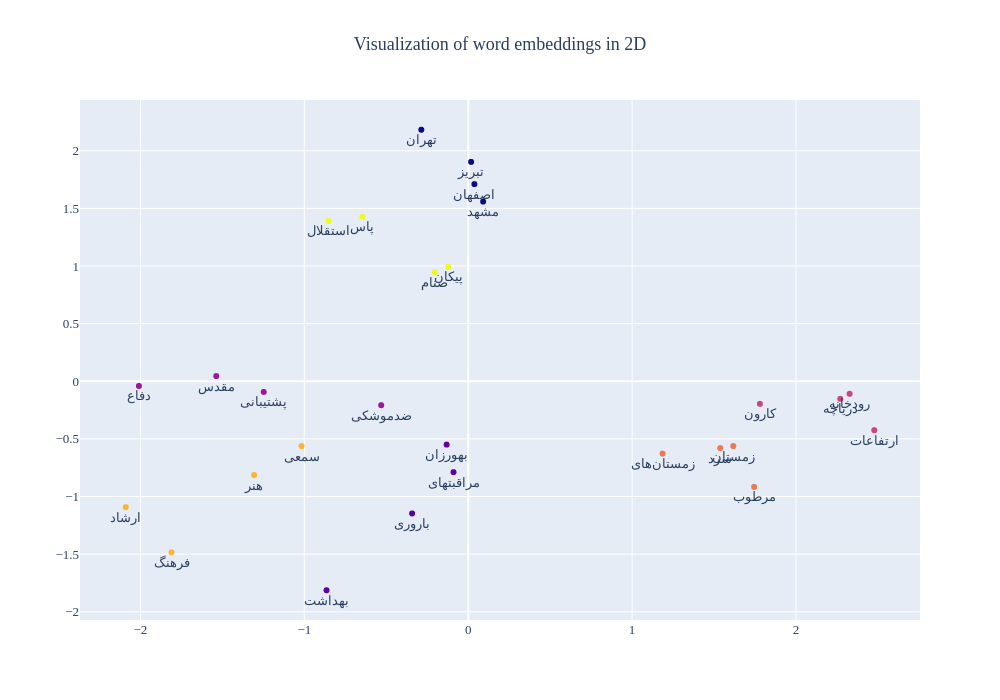
\includegraphics[width=\linewidth]{images/2d_embedding_similarity.png}
    \end{subfigure}
    \hfil
    \begin{subfigure}{0.45\linewidth}
        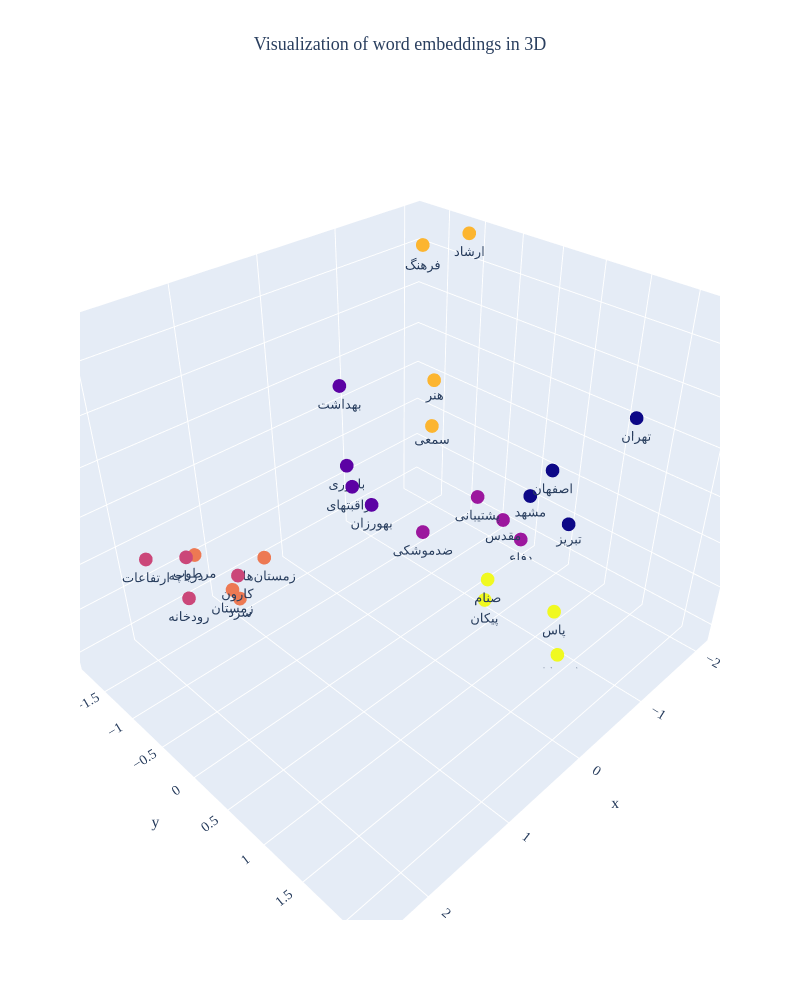
\includegraphics[width=\linewidth]{images/3d_embedding_similarity.png}
    \end{subfigure}
    \caption{نمودار تعبیه کلمات مدل با کاهش ابعاد به ۲ و ۳ بعد}
    \label{embedding_diagram}
\end{figure}

\pagebreak

\section*{بخش دوم}

\subsection*{گام اول}

در این سوال داده‌ها را به این صورت مدل کرده‌ایم که یک جمله به تمام تگ‌های \lr{POS} آن
به مدل داده می‌شود و انتظار داریم که مدل بر اساس تعبیه‌های کلمه خروجی \lr{POS} آن را تولید کند.
طبیعتا طول بعضی از جمله‌ها کمتر است به انتهای این جملات \lr{padding} اضافه می‌کنیم تا برای مدل
قابل آموزش باشد. در این حالت با توجه به توضیح داده‌ها که در شکل \ref{sentence_len_dist} آورده شده است،
می‌توان جملات با طول بیشتر از 100 را حذف کرد. چرا که علی‌رغم طول زیاد، فراوانی کمی دارند.

\begin{figure}[h]
    \centering
    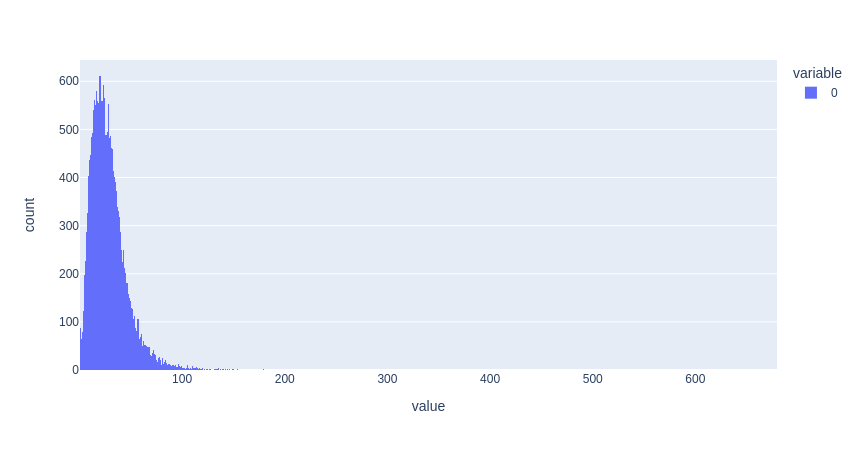
\includegraphics[width=0.8\linewidth]{images/distribution.png}
    \caption{نمودار توزیع اندازه طول جملات}
    \label{sentence_len_dist}
\end{figure}

نمودار کلی مدل در شکل \ref{lstm_architecture} آورده شده است. مدل \lr{GloVe} داده شده به صورت یک لایه
\lr{Embedding} آورده شده است. در ادامه خروجی لایه‌ تعبیه کلمه به لایه \lr{LSTM} داده شده و در ادامه با
استفاده از لایه \lr{Dense} خروجی نهایی مدل تولید می‌شود. این مدل در داده‌های آموزش و ارزیابی به صحت
$0.96$ و در داده‌های تست به صحت $0.93$ می‌رسد.

\begin{figure}[h]
    \centering
    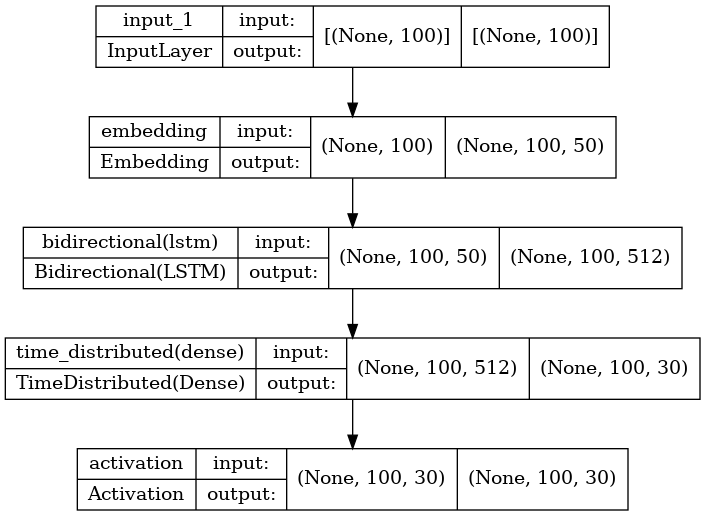
\includegraphics[width=0.8\linewidth]{images/architecture.png}
    \caption{ساختار کلی مدل \lr{LSTM}}
    \label{lstm_architecture}
\end{figure}

\subsection*{گام دوم}

در شکل \ref{acc_loss_epoch} نمودار خطای مدل بر روی داده‌های آموزشی و ارزیابی در هنگام طی هر گام یادگیری
آورده شده است. آموزش مدل در طی ۱۵ گام یادگیری و با نرخ یادگیری $10^{-3}$ انجام شده است.
در گام‌های نهایی آموزش، خطای مدل در داده‌های ارزیابی چندان تغییراتی نداشته در نتیجه
می‌توان گفت که آموزش مدل به حالت اشباع رسیده بوده است و ممکن بود که اگر آموزش
را بیشتر ادامه می‌دادیم مدل بر روی داده‌ها بیش‌برازش می‌شد. روند رشد نمودار صحت نیز
تقریبا به همان صورت است با این تفاوت که در گام‌هایی نهایی مدل همچنان به صورت بسیار ضعیف
در حال بهبود بوده است.

\begin{figure}[h]
    \begin{subfigure}{0.45\linewidth}
        \centering
        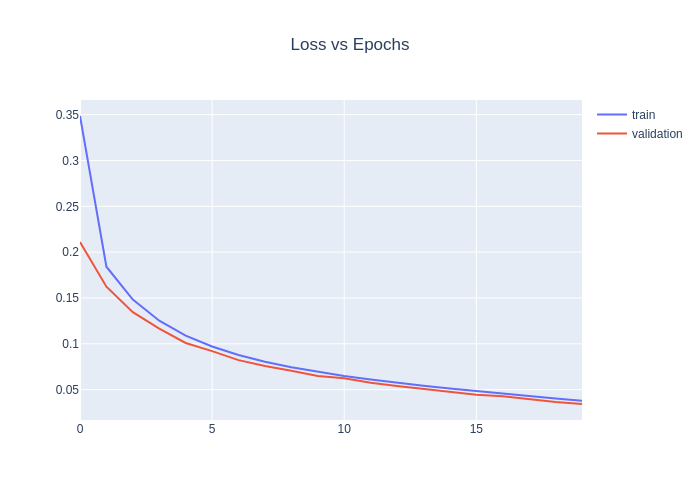
\includegraphics[width=\linewidth]{images/loss_epoch.png}
    \end{subfigure}
    \begin{subfigure}{0.45\linewidth}
        \centering
        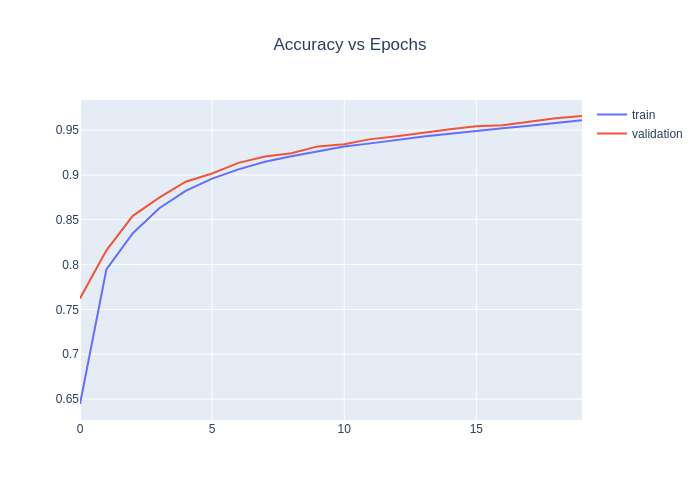
\includegraphics[width=\linewidth]{images/acc_epoch.png}
    \end{subfigure}
    \caption{نمودار تغییرات خطا و صحت در طی گام‌های مختلف یادگیری}
    \label{acc_loss_epoch}
\end{figure}

در شکل \ref{confusion_matrix} ماتریس درهم‌ریختگی مدل مشاهده می‌شود. همان‌طور که مشاهده می‌شود
درصد خوبی از تگ‌های \lr{DELM} برچسب \lr{CON} خورده است. دلیل
شباهت بسیار زیاد این دو برچسب است. هر دو این برچسب‌ها در انتهای جمله آمده و مشخص می‌کنند که
جمله قبلی به پایان رسیده است.
علاوه بر این مشکل، مدل برچسب \lr{N\_SING} را به اشتباه برچسب \lr{N\_PL} و \lr{ADJ} تشخیص می‌دهد.
برچسب زدن داده‌های \lr{N\_SING} و \lr{N\_PL} به جای یکدیگر به دلیل ساختار زبان فارسی و وجود کلماتی نظیر جمع مکسر
است که در ظاهر ساده هستند اما در واقع جمع هستند. همچنین درصد زیادی از داده‌های \lr{ADJ} برچسب
\lr{N\_SING} زده می‌شود. دلیل این مشکل نیز مشابه مشکل قبلی است. در فارسی عبارت‌های مضاف‌ و مضاف‌الیه و موصوف و صفت
بسیار شبیه به هم هستند در نتیجه طبیعی است که عبارت‌های اسمی و صفت به جای هم تشخیص داده شوند.

\begin{figure}[h]
    \centering
    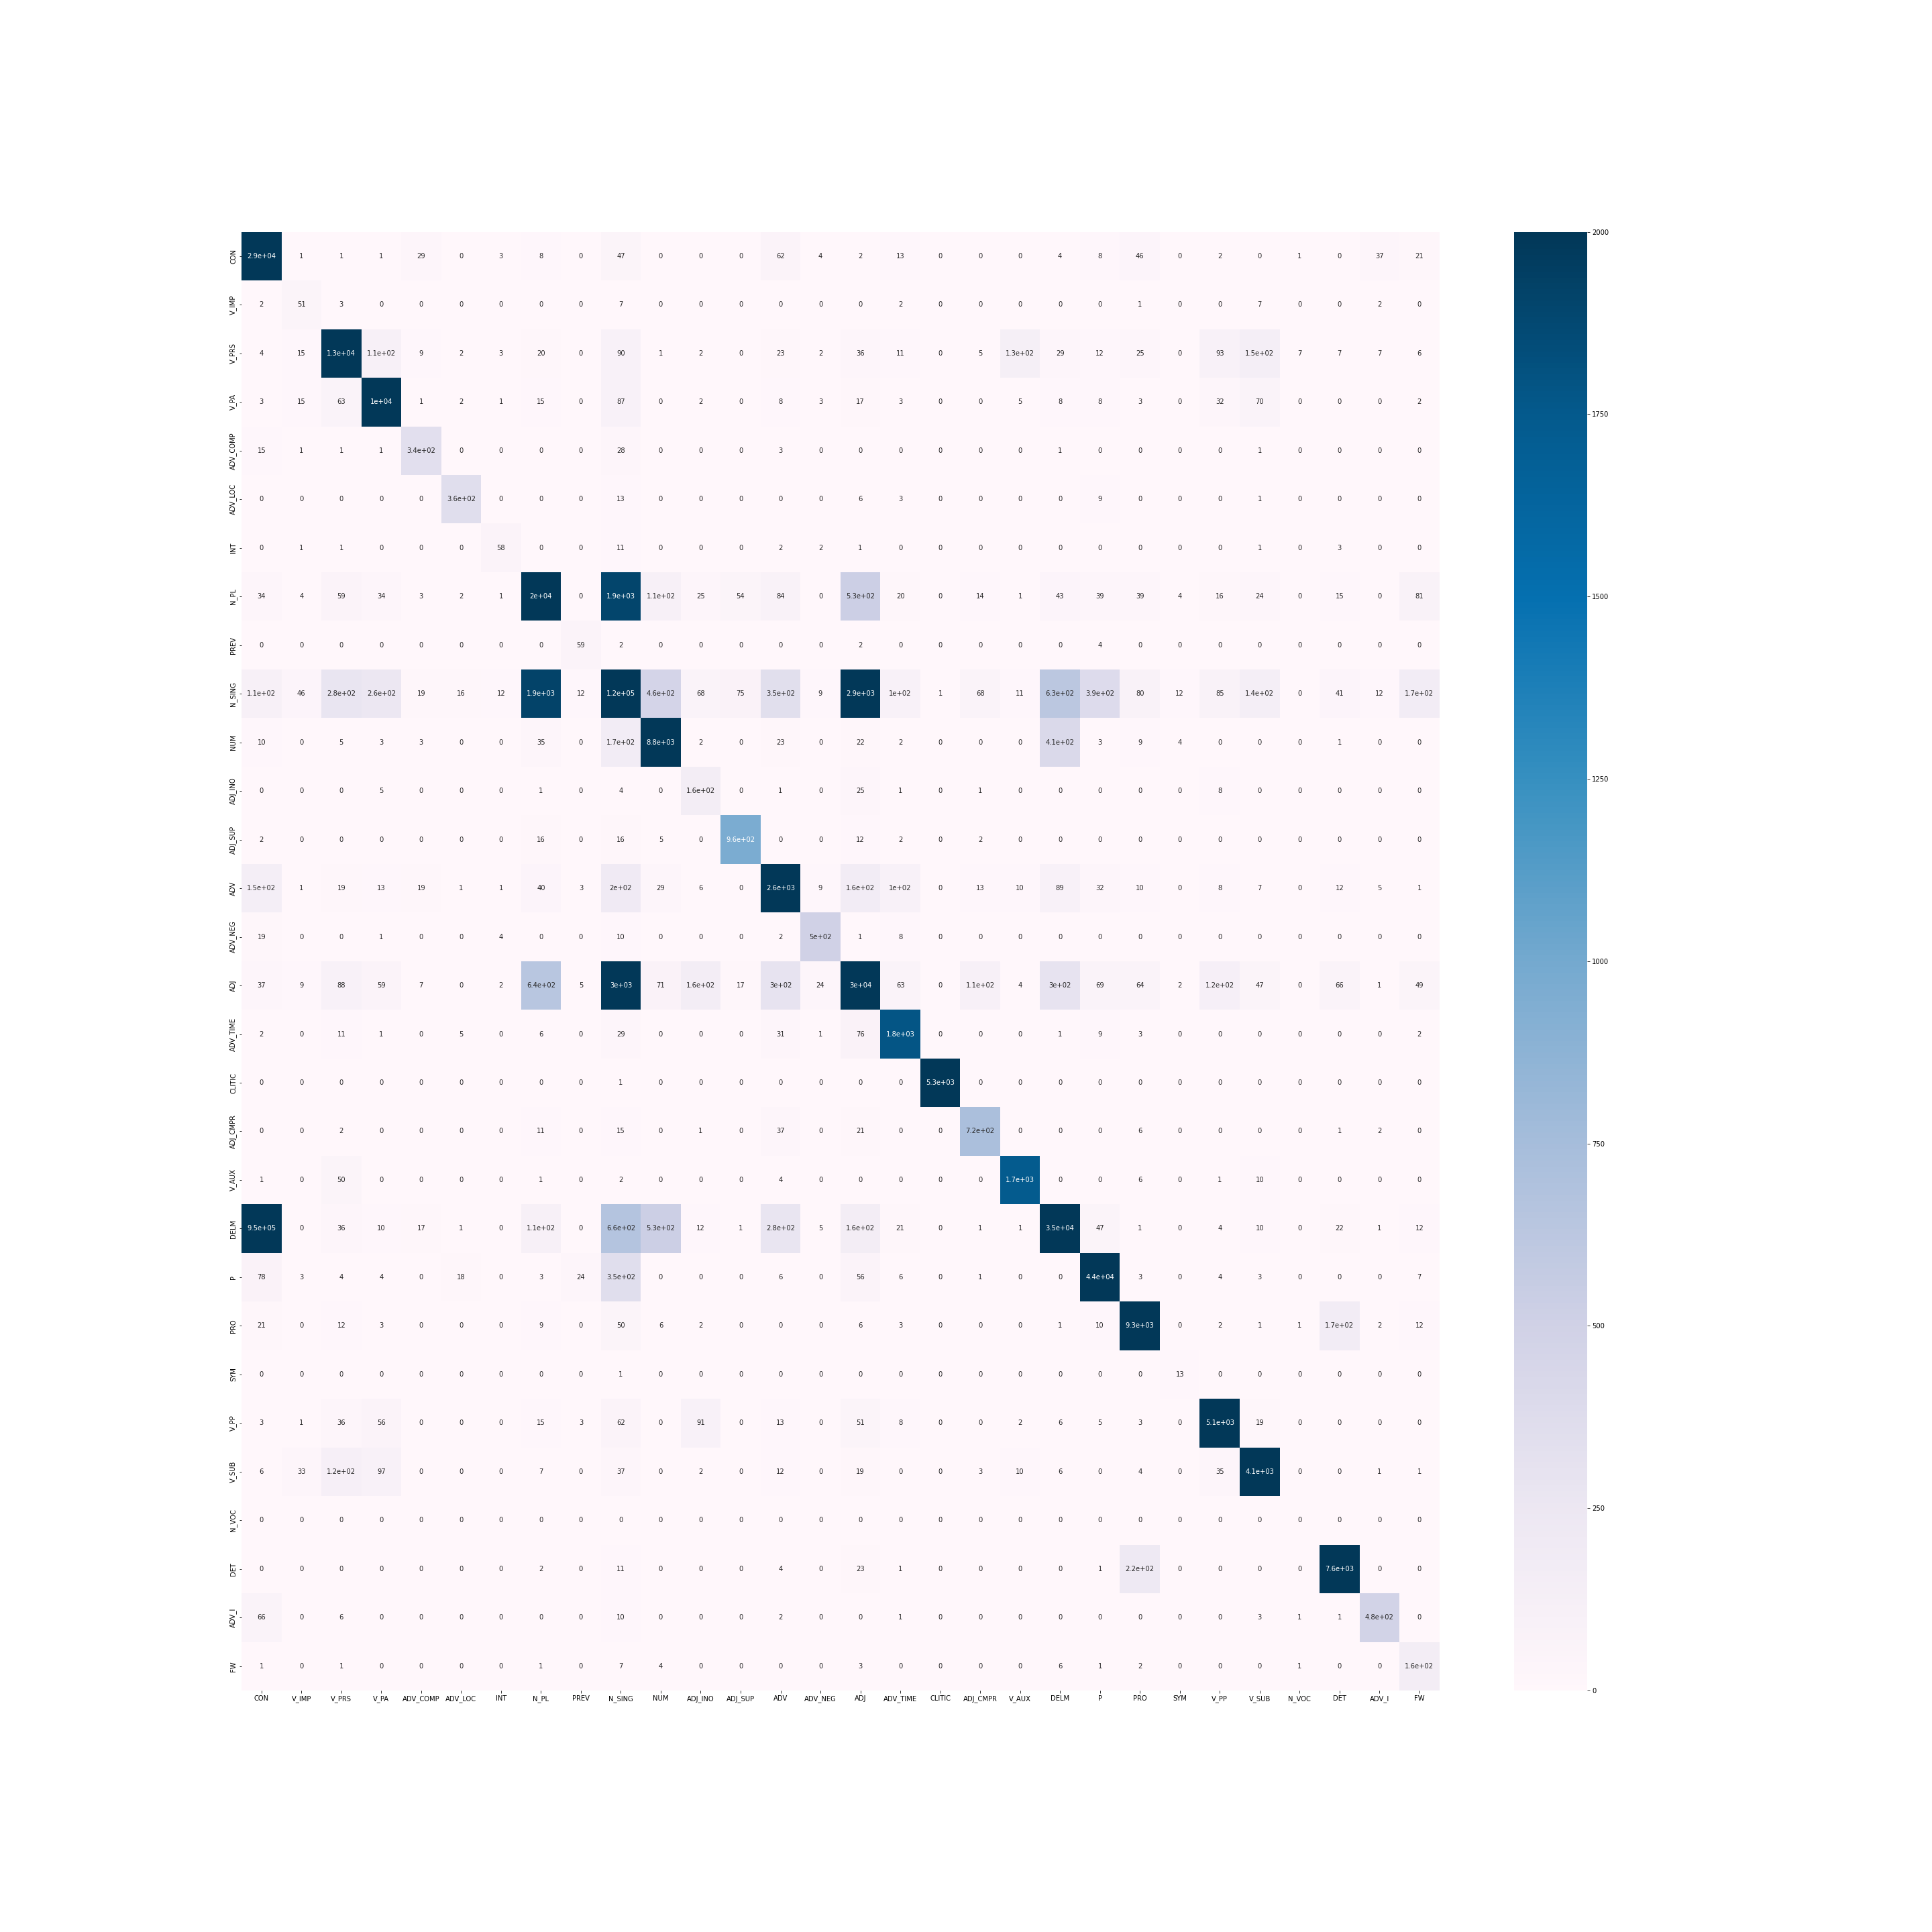
\includegraphics[width=0.8\linewidth]{images/confusion_matrix.png}
    \caption{ماتریس درهم‌ریختگی شبکه عصبی}
    \label{confusion_matrix}
\end{figure}

در نهایت در جدول \ref{tag_accuracy} درصد صحت تشخیص هر تگ آورده شده است. همان‌طور که مشاهده می‌شود به
جز تگ \lr{CON} برای باقی تگ‌ها معیار صحت ۱۰۰ درصد محاسبه شده است. این اتفاق گر چه در نگاه اول خوشحال‌کننده
است اما لزوما به معنی عملکرد بهینه مدل نیست. چرا که طبق جدول در‌هم‌آمیختگی که پیش‌تر رسم شد، مدل
مشکلات جدی دارد. با بررسی جدول درهم‌آمیختگی مشخص می‌شود که علت پایین بودن

\begin{latin}
\begin{table}[h]
    \centering
    \caption{\rl{جدول صحت تشخیص هر تگ} \lr{POS}}
    \label{tag_accuracy}
    \begin{tabular}{l|l}
        Tag & Accuracy \\ \hline
        CON & 0.28 \\ \hline
        V\_IMP & 1 \\ \hline
        V\_PRS & 1 \\ \hline
        V\_PA & 1 \\ \hline
        ADV\_COMP & 1 \\ \hline
        ADV\_LOC & 1 \\ \hline
        INT & 1 \\ \hline
        N\_PL & 1 \\ \hline
        PREV & 1 \\ \hline
        N\_SING & 0.99 \\ \hline
        NUM & 1 \\ \hline
        ADJ\_INO & 1 \\ \hline
        ADJ\_SUP & 1 \\ \hline
        ADV & 1 \\ \hline
        ADV\_NEG & 1 \\ \hline
        ADJ & 0.99 \\ \hline
        ADV\_TIME & 1 \\ \hline
        CLITIC & 1 \\ \hline
        ADJ\_CMPR: & 1 \\ \hline
        V\_AUX & 1 \\ \hline
        DELM & 0.28 \\ \hline
        P & 1 \\ \hline
        PRO & 1 \\ \hline
        SYM & 1 \\ \hline
        V\_PP & 1 \\ \hline
        V\_SUB & 1 \\ \hline
        N\_VOC & 1 \\ \hline
        DET & 1 \\ \hline
        ADV\_I & 1 \\ \hline
        FW & 1 \\
    \end{tabular}
\end{table}
\end{latin}

\end{document}